%----------------------------------------------------------------------------
\chapter{Előzmények}
%----------------------------------------------------------------------------

\section{A részfeladatok}

A diplomatervezés feladat keretein belül egy autonóm robot megtervezése és
megépítése volt a cél. Ez a feladat egy komplex tervezési feladat, amely több fő
részfeladatra bontható. A munkám során ezeket a részeket, mint kisebb önálló
részfeladatokat, egymás után oldottam meg, kisebb-nagyobb átfedésekkel. Ezeket a
részfeladatokat az alábbi módon határoztam meg:

\begin{itemize}
\item Hardver
  \begin{itemize}
  \item Mechanikai kialakítás megtervezése és kialakítása
  \item Szenzor és motor kiválasztása
  \item Energiaellátás megtervezése és kialakítása
  \item Motor és szenzorvezérlő áramkör megtervezése és kialakítása
  \item Magasabb szintű döntéshozó egység választás
  \end{itemize}
\item{Firmware}
  \begin{itemize}
  \item Motor és szenzorvezérlő áramkör firmware megtervezése és kialakítása
  \end{itemize}
\item{Software}
  \begin{itemize}
  \item Beágyazott Linux rendszer készítése
  \item ROS2 keretrendszer telepítése
  \item A robot hardver integrálása a ROS2 keretrendszerbe
  \item Demo alkalmazás elkészítése amelyben a robot labirintusban halad.
  \end{itemize}
\end{itemize}

\section{Az előzmények}

A feladat egyik központi részének alapját a robot alkotó elektronikai komponensek
jelentették. A feladathoz felhasználtam a korábbi, önálló laboratóriumi projekt
kereteiben elkészített áramköri paneleket, amelyek egy témában a diplomatervhez
nagyon hasonló alkalmazáshoz készültek. Ezek biztosították a hardveres alapot a
robot kialakítása során.  A robot koncepcióját bemutató következő fejezetben
részletesebben kitérek a panelek felhasználására és topológiájára, a jelen
fejezetben pusztán az elektronikai igényekről, specifikációkról valamint az
alkatrészek megválasztásáról lesz szó. A projekt verziókövetve megtalálható a
github repository-ban~\cite{RpirobotGitrepo}, ahol a \verb|pcbs| mappa alatt egy
\verb|movement-control| és egy \verb|power-supply-unit| könyvtárban találhatóak a
KiCAD projektek. Az ábrák pdf formátumban elérhetőek a
\verb|doc/schemas/circuits| mappában a \verb|ctrl-board| és \verb|pwr-supply|
mappákban.

\subsection{Motor és szenzor választás}

A robot két fő ponton kapcsolódik a környezetéhez amiben a feladatát ellátja: a
szenzoraival, és a motorjaival. Ezen alkatrészek kiválasztása a tervezési fázis
elején történt, és meghatározó szerepű volt.

\medskip

A szenzorok biztosítják az információszerzés lehetőségét a robot számára a
külvilág felől, így a pontos feladatvégrehajtáshoz megfelelő szenzor kiválasztása
elengedhetetlen.  Minden feladathoz szükséges a végrehajtáshoz szükséges
információk kinyerése a környezetből, ezeknek az információknak a tipusa eltérő
lehet. A navigációhoz nagyon gyakran alkalmazunk távolságmérést amivel a robot
relatív pozícióját vagy környezetének felépítését szeretnénk vizsgálni.  A
távolságmérésre többfajta bevált megoldás létezik mint például a radar, a szonár,
vagy esetleg a lidar. A robot esetében az olyan szenzorok kiválasztására volt
szükség, amelyekkel pontos távolságméréssel falak relatív pozícióját lehetett
meghatározni.

Rövid kutatás után az STMicroelectronics által gyártott VL53L1 szenzorchipekre
esett a választásom. Ezek a chipek LIDAR működésű érzékelők, azaz lézer
kibocsátásán és a visszaverődés érzékelésén alapul a működésük. Rendkívül gyakori
keresési találatok voltak, és sok hobbielektronikai projekt foglalkozott velük. A
kommunikáció a chippel I2C buszon zajlik, a szenzorok komplexitása és vezérlésük
bonyolultsága miatt, azonban használatukhoz a gyártó külön driver csomagot
biztosít. A gyártó nem csak integrált áramkör formájában forgalmazza ezeket az
alkatrészeket, hanem VL53L1-SATEL néven, mint modul is kaphatóak. Ebben a
kiszerelésben a táp- és földlábak, az I2C busz valamint két fontos láb, ki vannak
vezetve a panel oldalán található tüskesorra.  A panel 3.3V feszültséget igényel,
amiből a szenzor IC számára előállít egy alacsonyabb feszültségszintet. Ez a
projekt szempontjából ideális, mert nincs szükség még egy tápfeszültségszint
előállítására, valamint a csatlakozás és majd a mechanikus rögzítés is könnyebb
egy kész áramköri modul esetében.

\begin{figure}
  \centering
  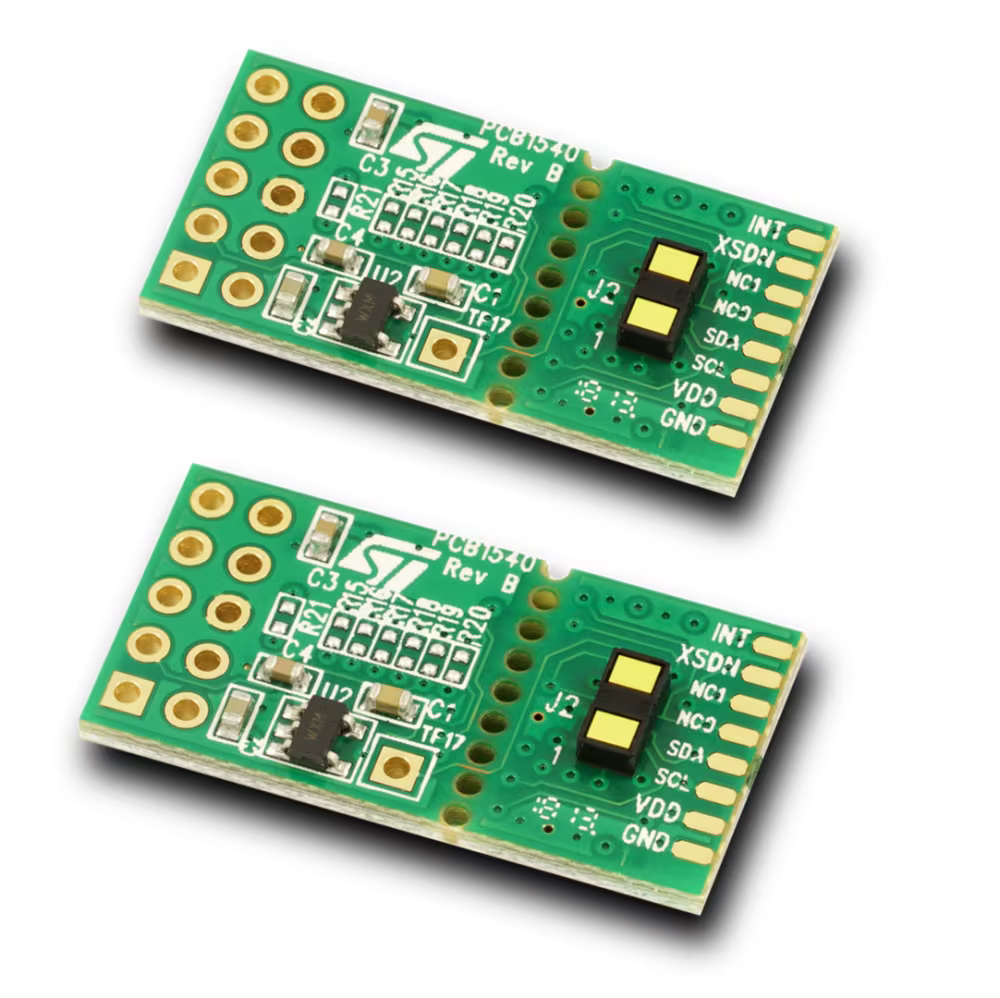
\includegraphics[width=100mm, keepaspectratio]{figures/ch1/vl53.png}
  \caption{A VL53L1-SATEL breakout board\cite{vl53l1source}}
  \label{fig:sensor}
\end{figure}

Az autonóm robot helyzetváltoztatása motorok segítségével történik. A motorok
meghatározásánál a feladat végrehajtásához szükséges teljesítmény és
forgatónyomaték igény, valamint a robot által leadható teljesítmény a két
legfontosabb paraméter. Fontos szerepet játszik továbbá a motor mehajtásának
módja, amely a kisebb robotok esetében szinte kizárólag DC motorok felhasználását
jelenti. A robot tervezése során fontos kiemelni, hogy a motor egyben érzékelő
is, ahhoz, hogy pontos beavatkozást végezhessünk, a motorok sebességének mérésére
is szükség van. A motorok sebességének mérésére leggyakrabban enkódereket
használunk, amiket néhány gyártó motorjaiban beépítve találunk, más esetekben
magunknak kell felszerelnünk azokat a motor tengelyére.

A projektben egyenáramú, szénkefés motorokat választottam, mert az ezekhez
tartozó feszültségszintet könnyen elő tudtam állítani, és teljesítményben
megfeleltek az alkalmazás számára. A motorok típusa N20E villanymotor, amelyet
könnyen be tudtam szerezni. Az alkatrészt kisméretű áttétellel szerelték fel, ami
a maximális elérhető fordulatszámot növelte a maximális nyomaték beáldozásával. A
kereskedő oldalán több különböző áttétellel felszerelt motor volt elérhető.  A
motor felfüggesztéséhez szükséges alkatrészek szintén elérhetőek voltak, ami nagy
segítségnek bizonyult a robot mechanikai megtervezése és realizációja során. A
motoron megtalálható volt továbbá egy inkrementális enkóder, amelyhez panelre
forrasztott tüskesoron keresztül lehetett áramkört illeszteni. Ezek a tárcsák \(2
* 7\) beosztást tartalmaztak. A motor 6V DC feszültségget igényel, a beépített
enkóder 3.3V-tól 5V-íg tetszőleges feszültségszinten tud működni, ami alkalmas a
projektben történő felhasználásra.

\begin{figure}
  \centering
  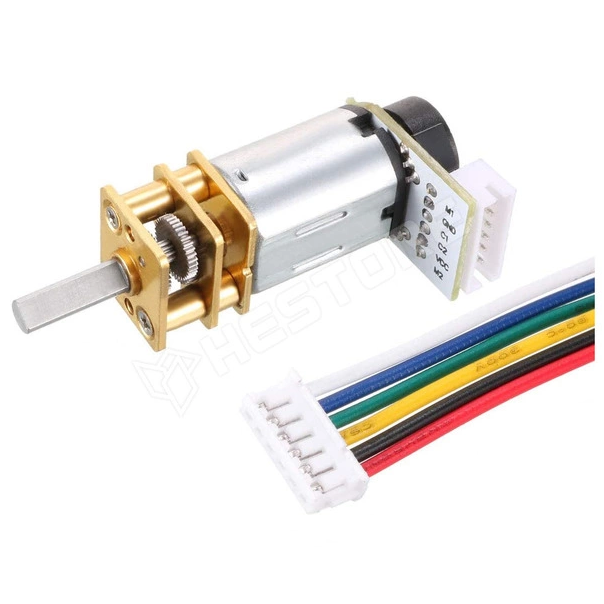
\includegraphics[width=100mm, keepaspectratio]{figures/ch1/motor.png}
  \caption{Az N20E motor\cite{n20emotor}}
  \label{fig:motor}
\end{figure}

\subsection{A tápellátás}

A robot különböző alkatrészeinek különböző tápfeszültségre van szüksége, az
alkatrészek hibamentes működéséhez elengedhetetlen egy stabil tápfeszültséget
biztosító eszköz.

Helyhezkötött alkalmazásokban ezt könnyedén megoldhatjuk a hálózati feszültség
felhasználásával, egy mobil alkalmazás esetén azonban ez nem megengedhető. Ilyen
esetben mobilis feszültségforrásra van szükség, amely lehet elem, vagy
akkumulátor. A projekt során az akkumulátoros megoldás mellett döntöttem, de
a moduláris kialakítás miatt ez könnyen módosítható konfiguráció.

\medskip

A táp megtervezése két fő paraméteren alapul: a szükséges teljesítményen, és az
igényelt tápfeszültségen. A szükséges feszültségszinteket az alkatrészek
függvényében a következőkben állapítottam meg:

\begin{itemize}
\item 5V:\@ a raspberry pi számára
\item 3.3V:\@ a vezérlőpanel, az enkóderek valamint a lidarok számára
\item 6V:\@ a motorok számára
\end{itemize}

A teljesítményviszonyokat pedig felülbecsléssel állapítottam meg. A vezérlés és
a Raspberry Pi teljes kihasználtság esetén 15W teljesítménynél kevesebbet
fogyaszt, ezért a pi irányában 15W teljesítményt írtam elő. A motorok szintén
15W-nál kevesebb teljesítményt vesznek fel a teljes kihasználáskor, ezért a motor
irányába menő teljesítményt szintén 15W-ban írtam elő.

A teljesítményáramlás a tápfeszültségek szempontjából a következőképpen alakul:
A Raspberry Pi, és a vezérlés rendre 5V és 3.3V tápfeszültségeket és 15W
teljesítményt kapnak. A motor egy vonalon kap összesen 15W teljesítményt és 6V
tápfeszültséget. Ez összesen egy 30W teljesítményt leadó feszültségforrást
igényel, valamint egy ehhez a teljesítménykonfigurációhoz méretezett tápot.

A tápellátó áramkör feladata a rendszer minden komponensét elegendő
teljesítménnyel ellátni. Ehhez a fent részletezetteknek megfelelően, olyan
tápáramkörre van szükség amely a következőket biztosítja: három kimeneti
tápfeszültségszint: 3.3V, 5V, 6V teljes rendszer
teljesítmény: 30W amely két részben oszlik meg: 15W a
6V kimenetre és 15W a 3.3V és 5V kimenetekre.
Ehhez rendelkezésre áll egy akkumulátoros feszültségforrás, amely a projekt
esetében egy Li-ion akkumulátorblokkot jelent. Ennek az akkumulátorblokknak a
kimenő teljesítménye alulról becsülhető 30W-al. A megfelelő feszültségek
előállításához három cellát használok, amelyek teljesen feltöltött állapotban
összesen 12.6V (\(3 * 4.2\)) feszültséget állítanak elő.

\medskip

A lítium cellák vezérlése egy komplex feladat, amely túlmutat a projekt céljain
és specifikációján, így egy megvásárolható BMS modult használtam. A
BMS\footnote{BMS:~Battery Management System} egy olyan modul amely a Lítium-ion
cellák vezérléséért felel, amely komplex elektronikát igényel. Három bemenetére
egyesével egy cella kapcsolódik, amelyek között kiegyensúlyozza a terhelést és
kimenetén 12V egyenfeszültséget állít elő.

A tápáramkör bemenete tehát 12V egyenfeszültség amiből a kívánt feszültségeket
kell előállítani. 

\medskip

A tápáramkör kialakításában a táp topológiája egy döntő fontosságú paraméter.
Kapcsolóüzemű tápok kialakításukat tekintve komplexebb és alkatrészigényesebb
architektúrák, amik kimenetén rendszerint valamennyi zaj jelenik meg a
kapcsolóüzemű mivoltukból kifolyólag. Ezeknek a tápegységeknek azonban hatalmas
előnyük a magas hatásfok, és az alacsony vesztességek.

Felhasználható eszközök még a feszültségstabilizátor áramkörök, amelyek rendkívül
stabil és zajmentes kimeneti feszültséget állítanak elő, ellenben a fölösleges
teljesítményt eldiszcipálják, így ez sokkal kisebb hatásfokú megoldás, ha nagy
feszültségkülönbségek között kell váltani.

A fenti feltételek alapján a felhasznált tápáramkör panel két kapcsolóüzemű
tápáramkört használ, hogy a 12V bemeneti feszültségből 6V és 5V feszültségeket
állítsanak elő. Ezek a kapcsolások nagyon gyakran fordulnak elő így az integrált
áramkör gyártója az adatlapban mellékelt referencia kapcsolást a jellemző
feszültségszintekre. A buck konverterek kimenetét kondenzátorokkal szűrtem, hogy
a kimeneten minél kevesebb zaj tudjon csak megjelenni.

Az 5V kimenő feszültségből egy LDO segítségével áll elő a vezérlőpanel és
enkóderek számára a 3.3V tápfeszültség. Ezzel a konstrukcióval minimalizáltam
a vesztességet, ami az LDO-n diszcipálódó teljesítményből adódna. 

Az áramkört az open source és Linux alatt is elérhető KiCAD programban
készült, a kapcsolási rajz az alábbi ábrán látható.

\begin{figure}
  \centering
  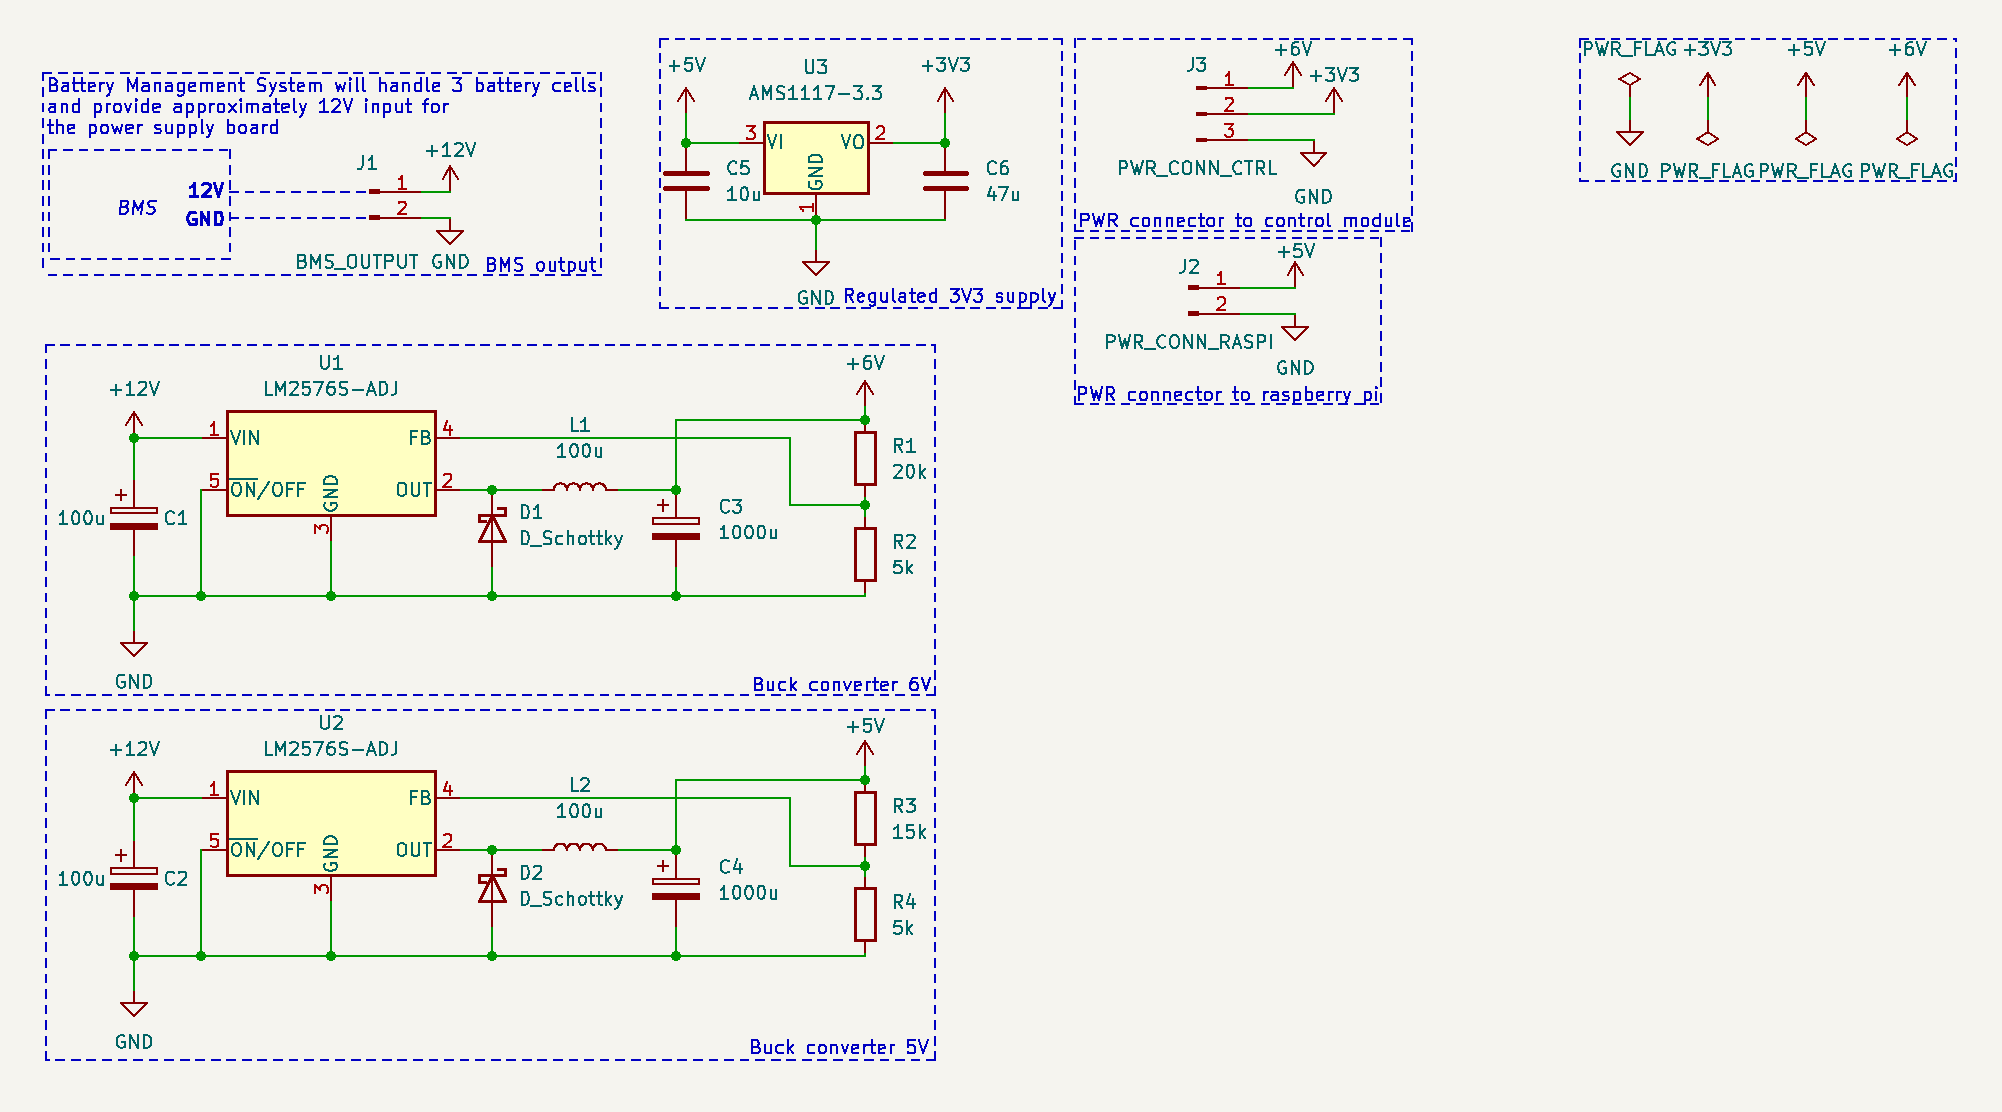
\includegraphics[width=100mm, keepaspectratio]{figures/ch1/power-supply-unit-schematic.png}
  \caption{A tápáramkör kapcsolási rajza}
  \label{fig:pwr_schematic}
\end{figure}

A kapcsolóüzemű tápáramörök kialakításnál jó gyakorlat, ha mezőkitöltéseket
használunk, amelyek jó hatással vannak a tápáramkör zajmentességére. Ezt
szemlélteti az alábbi ábra a tápáramkör layoutjáról.

\begin{figure}
  \centering
  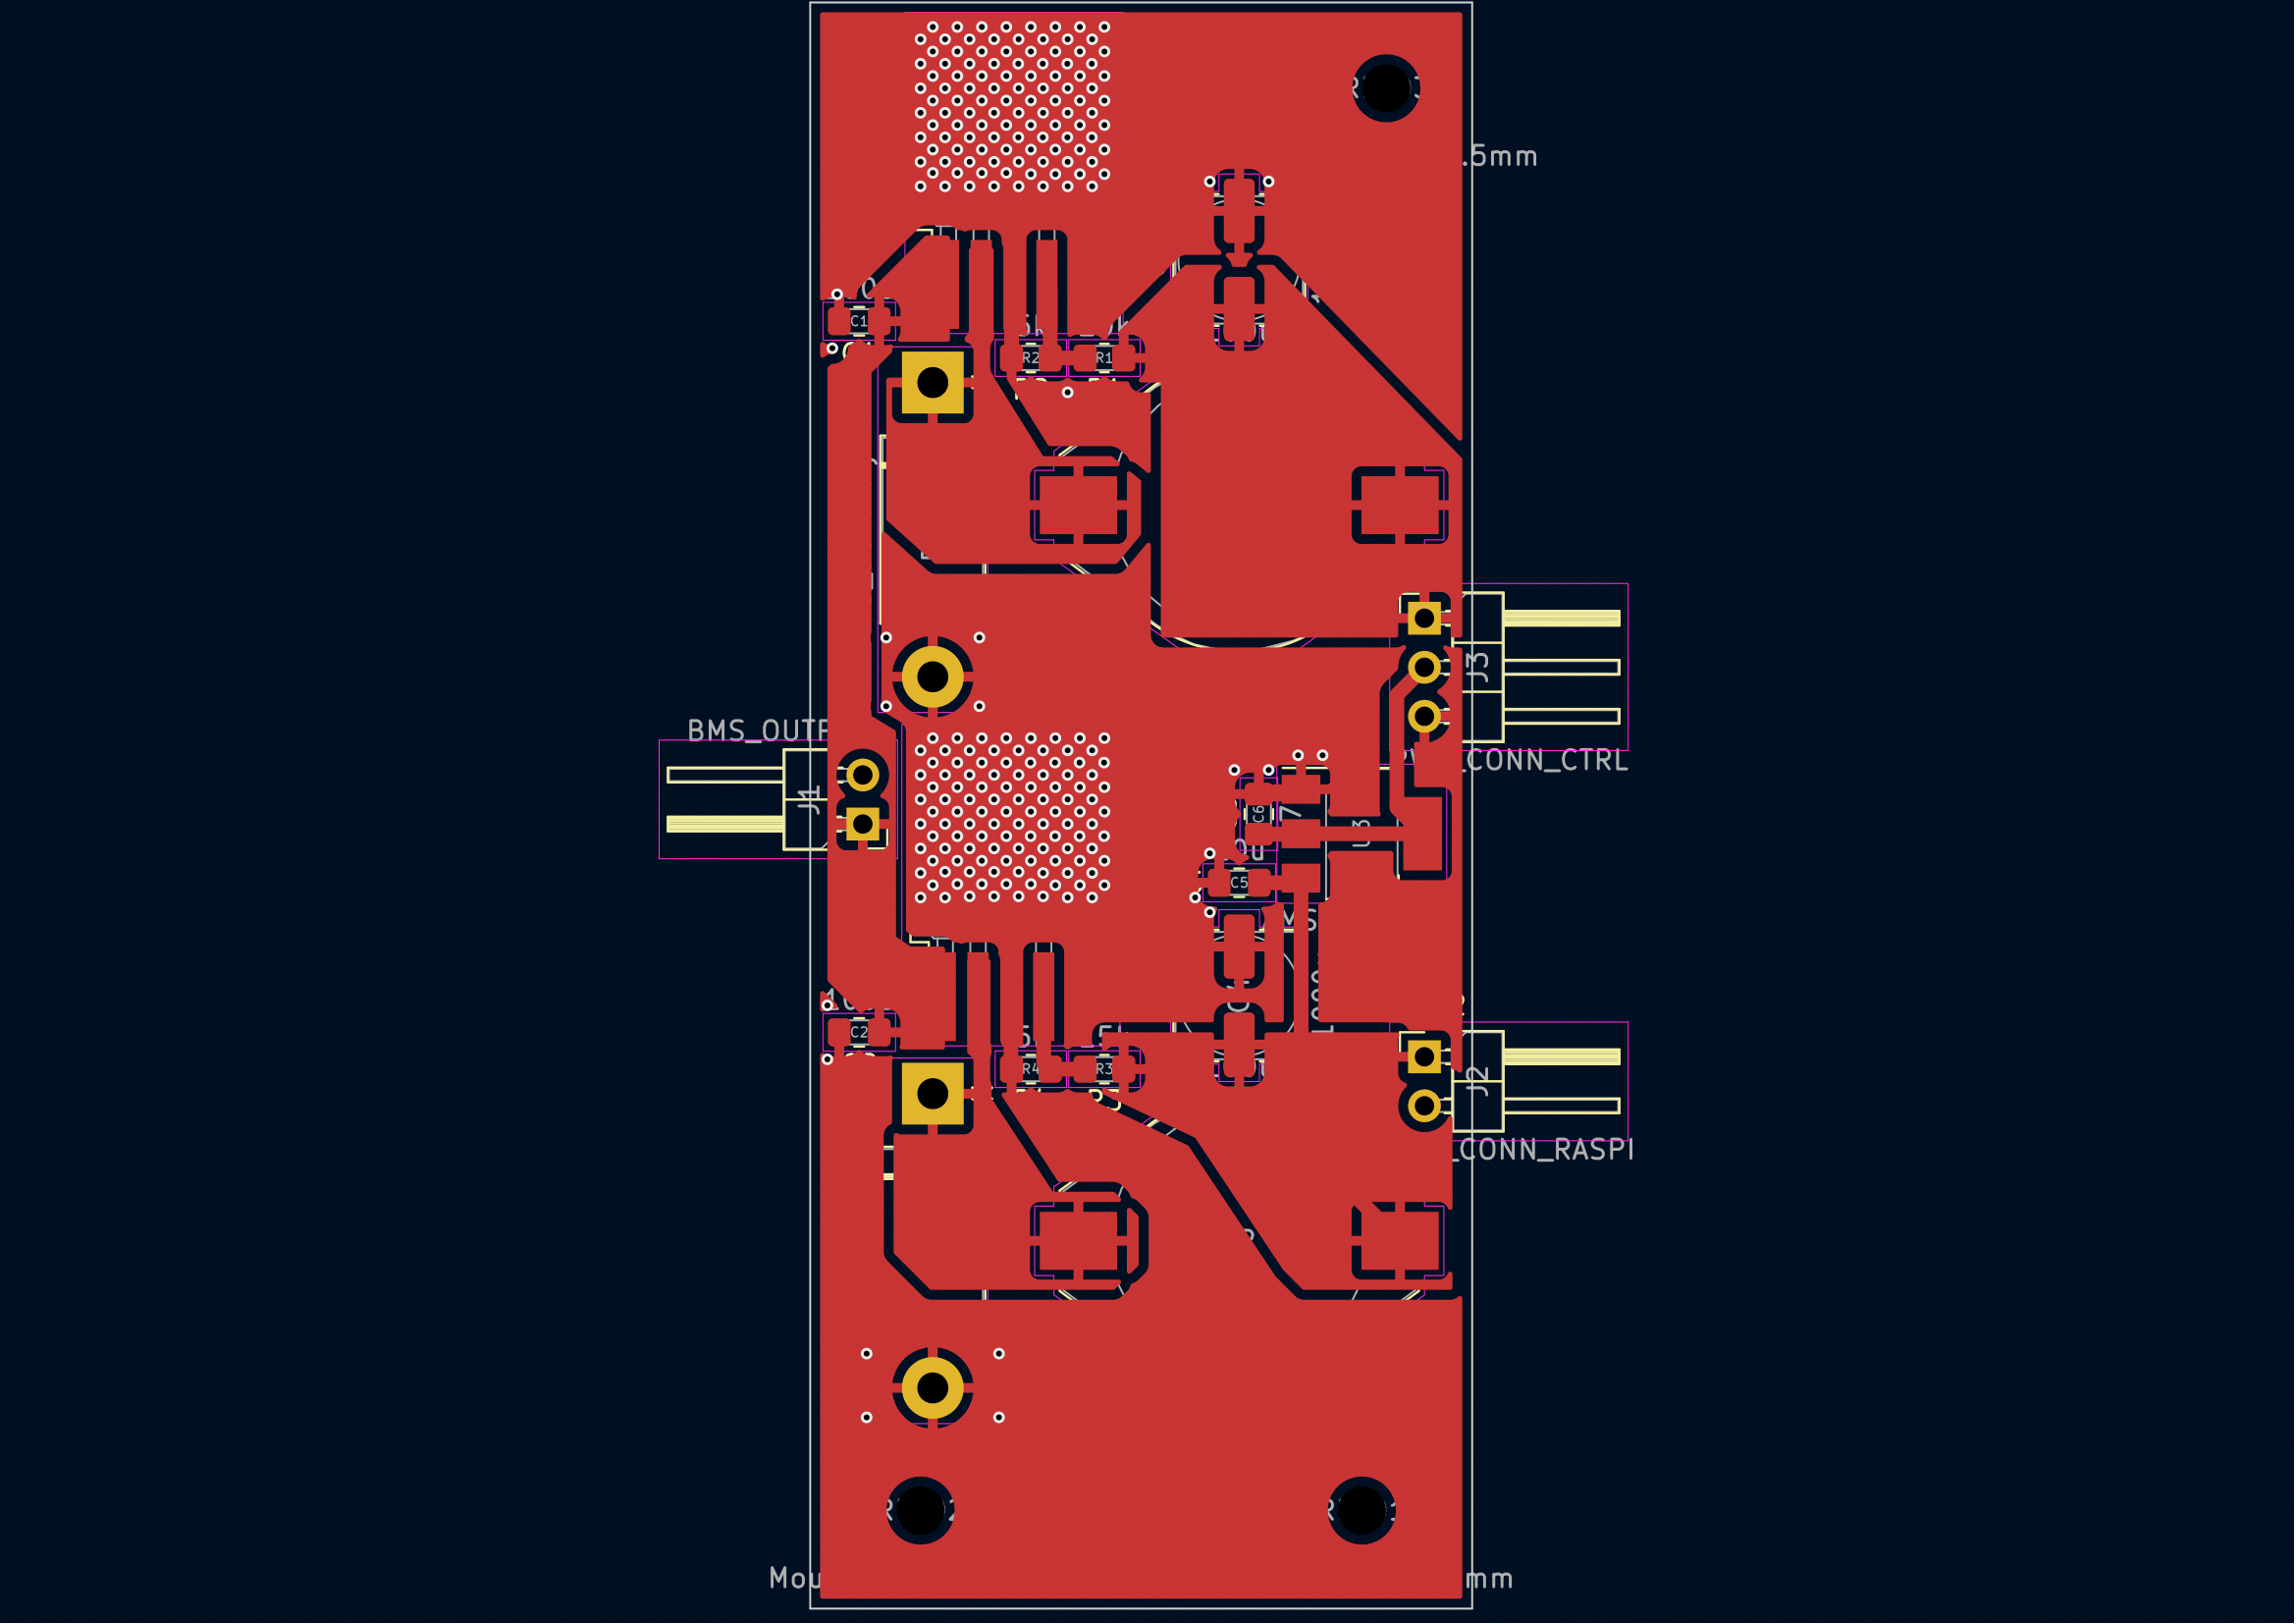
\includegraphics[width=100mm, keepaspectratio]{figures/ch1/power-supply-unit-layout.png}
  \caption{A tápáramkör layout képe}
  \label{fig:pwr_layout}
\end{figure}

\subsection{A vezérlő elektronika}
A tápáramkör bemutatása után következzen a vezérlőpanel bemutatása. Ennek a
panelnek az elsődleges feladata, hogy a robot motorjait vezérelje, valamint
a szenzorait inicializálja és olvassa.

Ez a panel egy mikrovezérlőt hordoz, amely mindezen funkcionalitást képes
ellátni. A használt kontroller egy STM32F103CB mikrovezérlő, amely egy
ARM Cortex-M3 maggal 20 kB RAM-mal, és 64 kB flash memóriával rendelkezik.

Az STM32 mikrovezérlőcsalád különösen elterjedt az autóiparban, és nagyon
népszerű termék. A vezérlő kiválasztásánál fontos szerepet játszott, hogy már
volt tapasztalatom STM32 mikrovezérlővel.

\medskip

A vezérlő feladatai közé tartozik, hogy a motorok meghajtását elvégezze. A
mikrovezérlő GPIO lábainak maximális árama nem elegendő a motor meghajtásához,
valamint feszültsége is elenyésző a motor szükségleteihez viszonyítva. Ebből a
célból egy-egy H-bridge áramkör kapott helyet a vezérlőpanelen, amelyet 3.3V
feszültségszintekkel lehet vezérelni, de a motor kimeneteire már képes 6V
feszültséget és a hozzá tartozó 15W teljesítményt kapcsolni. A H-híd topológia
előnye, hogy a motor mindkét irányba vezérelhető lévén a polaritás megfordítható
a H-bridge megfelelő vezérlésével. A meghajtó áramkörök teljesítmény bemenetére
csatlakozik a tápáramkör által előállított 6V.

Lévén a motorok enkóderrel is fel vannak szerelve, így a mikrovezérlő mérheti
ezen motorok sebességét, és ezzel egy esetleges szabályzási kör megvalósítása is
lehetővé válik. A motorok szögsebessége ezen felül szintén egy fontos információ
a magasabb szintű logika számára is.

További fontos feladata a vezérlőnek, hogy a távolságmérő szenzorokat
periodikusan olvassa, és ezek értékét eltárolja. Ez később a felsőbb szintű
logika számára lehet fontos információ, valamint extra védelmet jelenthet, ha a
vezérlő le tudja fékezni a robotot, ha egy adott küszöbérték alatt mér egy
szenzorral, így elkerülve egy lehetséges ütközést. Ehhez a szenzorokat egy I2C
buszra kell csatlakoztatni, amelyet a mikrovezérlő meghajt. A panelen a
szenzorokhoz egy egy GPIO által vezérelt nyomvonal is vezet, amely az egyedi
címkiosztás miatt lesz majd fontos.

Végül de nem utolsó sorban a vezérlő feladata, hogy a már említett felsőbb szintű
logikát végrehajó Raspberry Pi-vel tartsa a kapcsolatot, és interfészt
biztosítson számára. Erre két lehetőség is van a boardon, az egyik a debug usart
port amely végül felhasználásra kerül majd, valamint egy külön I2C port, ami a
panelre ki van vezetve.

A vezérlőpanelen továbbá helyet kapott egy steppper motor meghajtó modul
foglalata is, ez viszont a diplomaterv során nem került kihasználásra.

\begin{figure}
  \centering 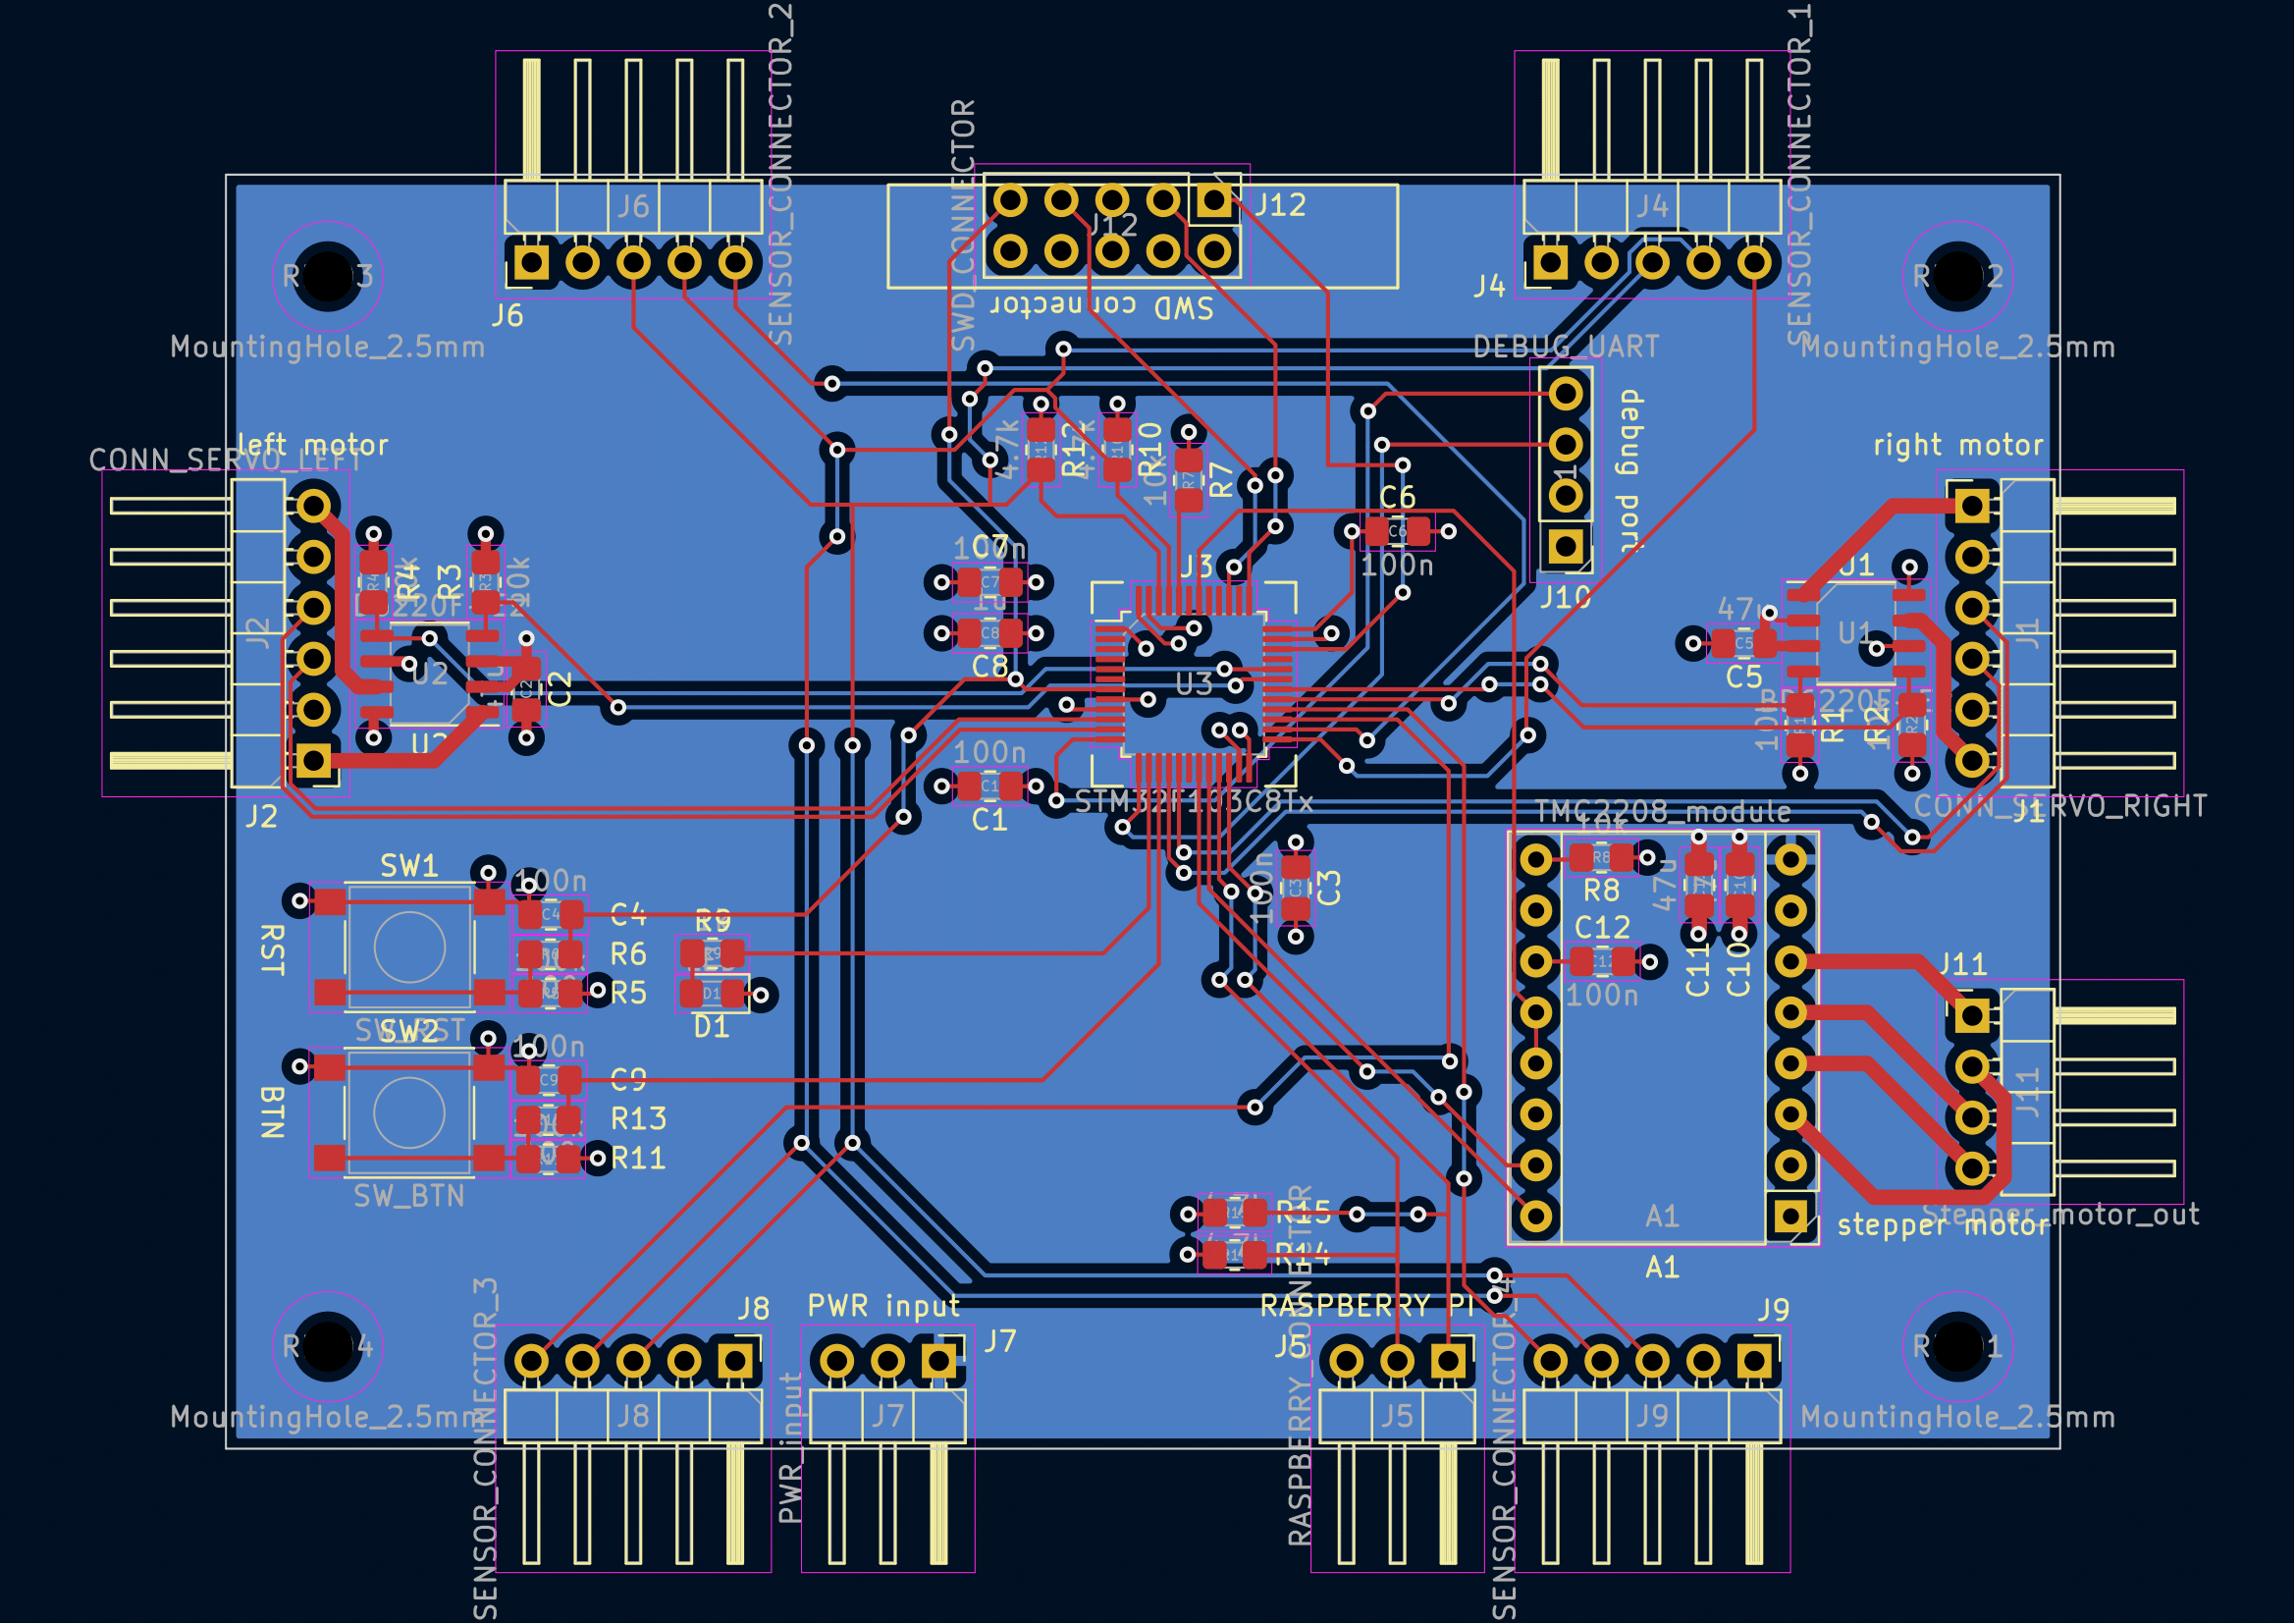
\includegraphics[width=100mm,
    keepaspectratio]{figures/ch1/movement-control-layout.png}
  \caption{A vezérlőpanel layout képe}
  \label{fig:crtl_layout}
\end{figure}

\begin{figure}
  \centering 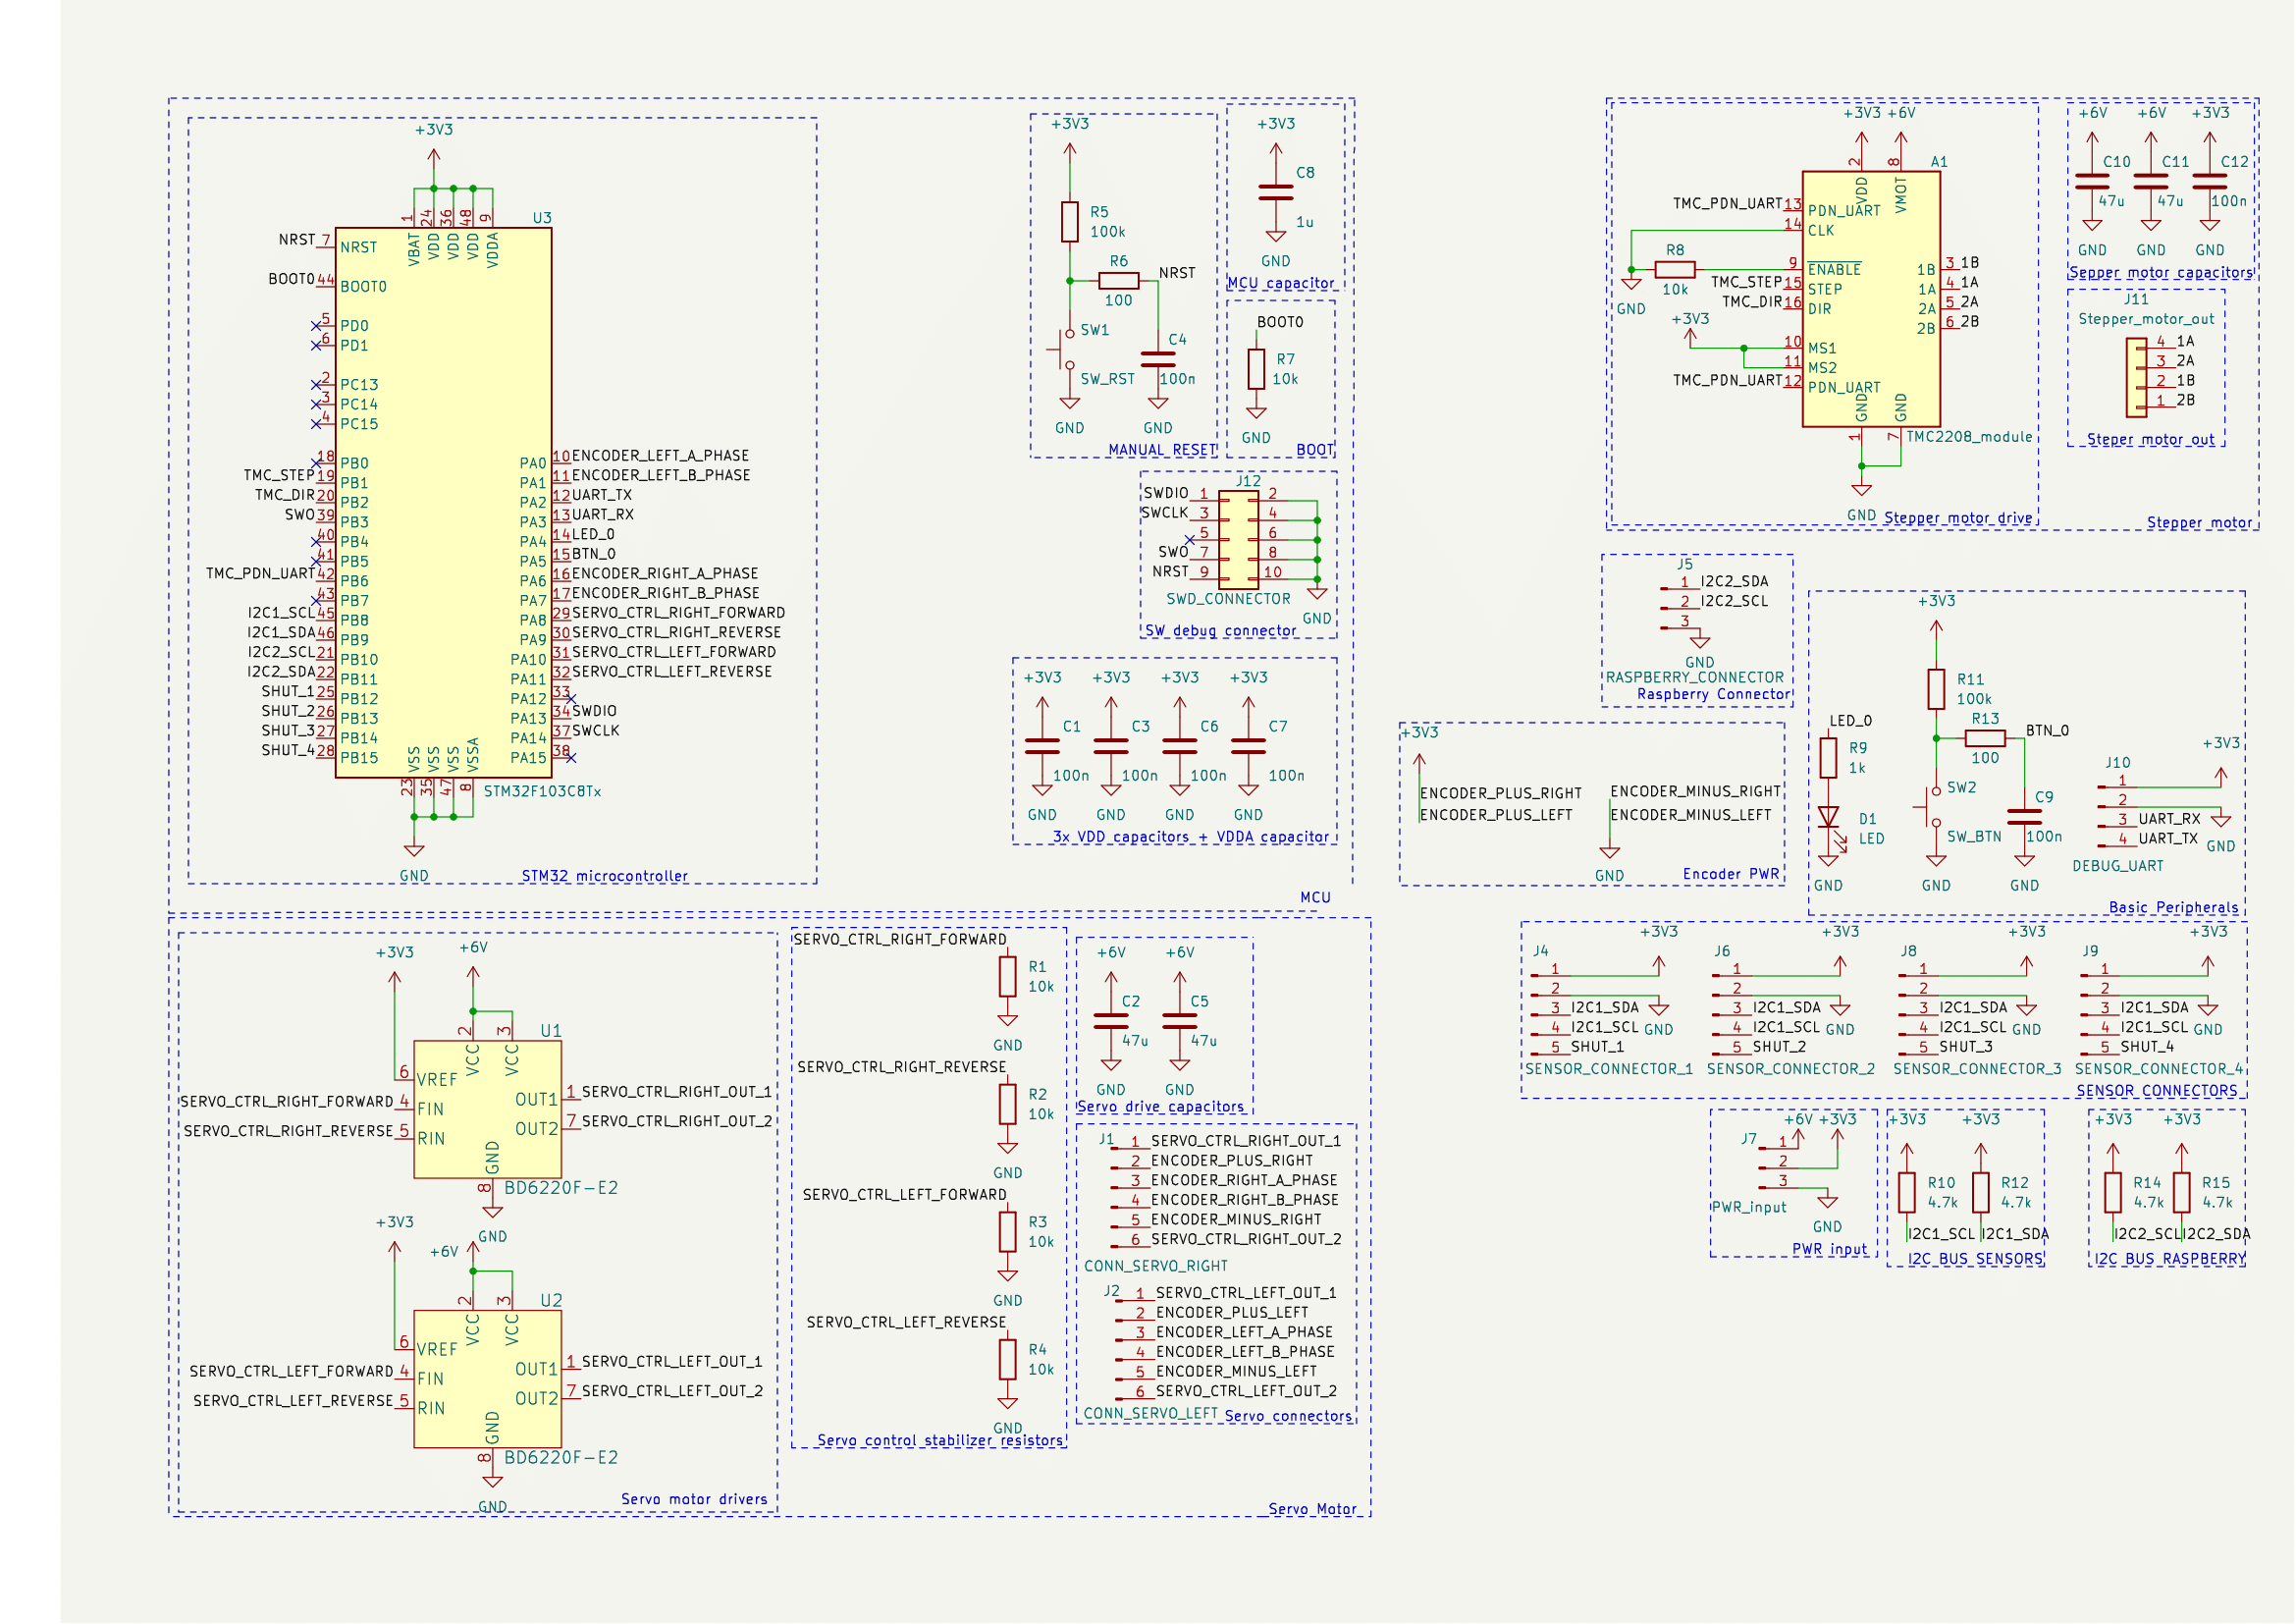
\includegraphics[width=100mm,
    keepaspectratio]{figures/ch1/movement-control-schematic.png}
  \caption{A vezérlőpanel kapcsolási rajza}
  \label{fig:ctrl_layout}
\end{figure}

A panel a~\ref{fig:ctrl_connectors} ábrán látható. Az ábrán a panel komponenseit
számmal jelöltem, az adott alkatrész vagy csatlakozó így beazonosítható:
\begin{enumerate}
\item Motor csatlakozó (bal oldal)
\item Motor csatlakozó (jobb oldal)
\item H-bridge (bal oldal)
\item H-bridge (jobb oldal)
\item Mikrovezérlő
\item Gombok és LED
\item Programozókábel csatlakozó
\item Legacy Raspberry Pi I2C csatlakozó
\item Tápcsatlakozó
\item Legacy léptetőmotor csatlakozó
\item Szenzor I2C csatlakozó (bal oldal)
\item Szenzor I2C csatlakozó (jobb oldal)
\item Szenzor I2C csatlakozó (első)
\item Szenzor I2C csatlakozó (hátsó)
\item USART csatlakozó
\end{enumerate}

\begin{figure}
  \centering 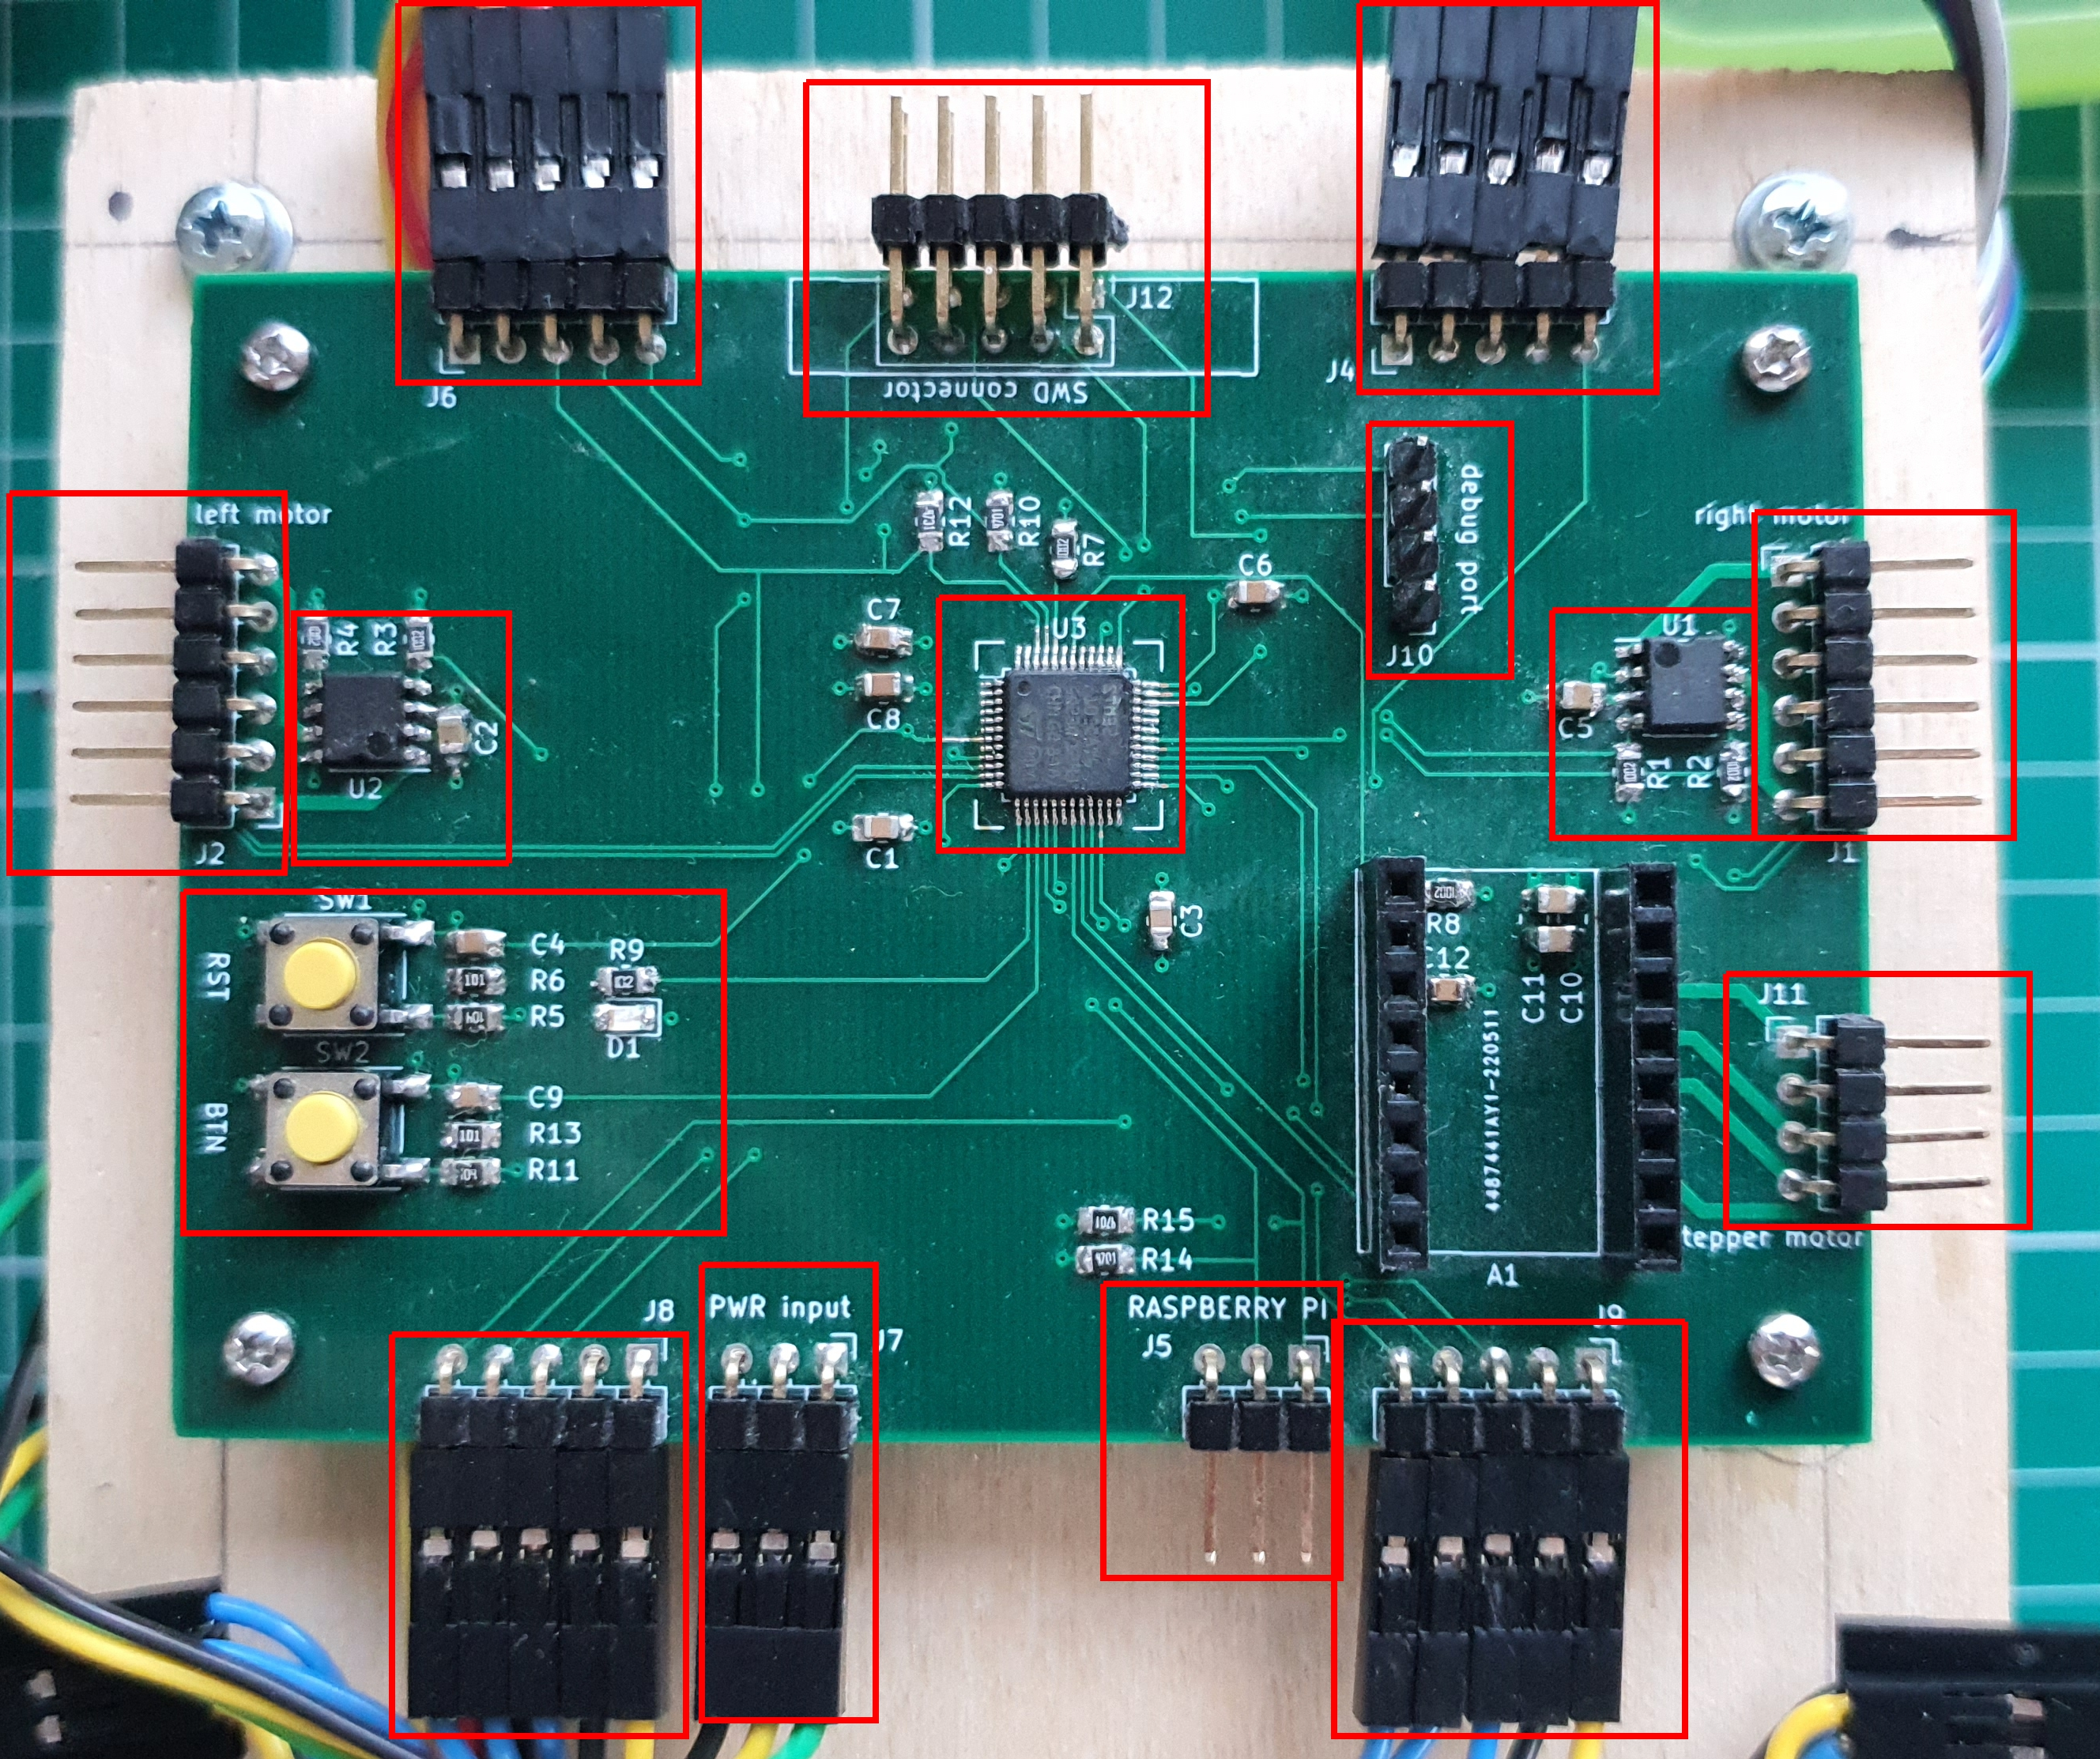
\includegraphics[width=100mm,
    keepaspectratio]{figures/ch1/control-connectors.png}
  \caption{A vezérlőpanel csatlakozási pontjai és komponensei}
  \label{fig:ctrl_connectors}
\end{figure}

\subsection{A robot magasabb szintű vezérlése}
A magasabb szintű funkcionalitás megvalósítása több számítási kapacitást igényel,
minthogy mikrovezérlőn könnyen implementálható legyen. A legtöbb robot ezen
célból a mikrovezérlőket egyes alrendszerek menedzselésére használja, és a
nagyobb teljesítményt igénylő általános feladatokat egy központi vezérlőegység
végzi. Egy ilyen áramkör panelre ültetése azonban nagy szakértelmet és komplex
panelt igényel, így alternatív megoldásra van szükség.

A magasabb szintű logikát végző processzorhoz, egy SBC\footnote{SBC:~Single Board
Computer}-t használtam. Ezek a panelek egy nagyteljesítményű processzort, vagy
SoC\footnote{SoC:~System On a Chip}-ot hordoznak, amelyet így könnyebben
intergrálhattam a robot rendszerébe. A választott SBC egy Raspberry Pi 4 B
modell, amelyet széleskörűen alkalmaznak hobbielektronikai megoldásokban, és
ipari felhasználásra is van példa. Ennek a boardnak könnyen hozzáférhető
dokumentációja van és rendelkeztem már tapasztalattal az eszközt illetően.

\section{Az elvégzendő feladatok}

Az előző szekcióban összefoglaltam a robot hardveres kialakítását, valamint a
felhasznált modulokat és alkatrészeket. A következőkben összefoglalom, a
diplomaterv során megvalósítandó célokat, és röviden ismertetem a
problémaköröket.

\subsection{Mechanikai tervezés és kialakítás}

Az egyetlen elvégzendő mechanikai feladat a robot mechanikai vázának
megtervezése, kialakítása, majd a robot végső összeszerelése. A váz megtervezése
során fel kell mérni, hogy milyen anyagok állnak rendelkezésre, megmunkálhatóság
illetve beszerezhetőség szempontjából, és milyen anyagokat célszerű választani a
robot feladata és motorjainak függvényében. A tervezés során figyelembe kell
venni az elektronikai alkatrészek topológiáját, és egy megfelelő struktúrát kell
kialakítani amely az összeszerelést és a majdani esetleges hibakeresést, vagy
alkatrészek cseréjét minél kevésbé nehezíti meg.

A váz feladata a robot struktúrális szilárdságának biztosítása, az elektronika
hordozása és védelme. A projekt során a robot prototípus modelljét készítettem
el, így a mechanikai tervezésre kisebb hangsúlyt fektettem.

A következő fejezetben röviden bemutatásra kerül a robot mechanikus váza, a
választott anyagok és alkatrészek.

\subsection{Firmware fejlesztés}

A vezérlőpanel egy mikrovezérlőt tartalmaz, mint központi elem, így a projekt
egyik központi feladata a mikrovezérlőn futó kód, a firmware fejlesztése. A

fejlesztés szerves része a megfelelő toolchain kiválasztása, a fejlesztéshez és
használt eszközök, összegyűjtése, és a munkakörnyezet kialakítása. Ezt követően a
firmware architektúrájának megtervezése következik. Ebben a lépésben a zajlik a
firmware feladatainak specifikálása, operációs rendszer szükségességének
felmérése, a szükséges keretrendszerek, könyvtárak kiválasztása. Ezekről
praktikusan dokumentáció és ábra készítése, majd a firmware funkcióinak
implementálása és tesztelés.

A vezérlőpanel, így a firmware feladatait a következő pontokban határoztam meg:

\begin{itemize}
\item A motorok meghajtása
\item A motorsebességek mérése, esetleg motorszabályozás
\item A szenzorok inicializálása és olvasása.
\item Interfész biztosítása amelyen keresztül a robot vezérelhető
\end{itemize}

\subsection{Embedded Linux image készítése}

A magasabb absztrakciós szinten megvalósítandó logikának elengedhetetlen
feltétele, egy megfelelő platform megléte. Ez a platform beágyazott környezetben
rendszerint Linux alapú operációs rendszert jelent. A feladat végrehajtásához
ezért szükséges egy ilyen operációs rendszer létrehozása, amelyhez többfajta
build környezet felhasználható.

A projekt következő feladata tehát egy Linux image létrehozása, ami támogatja a
célplatformot. Ennek az imagenek tartalmaznia kell minden olyan szoftveres
komponenst és konfigurációt, hogy a rendszer bootolásra alkalmas legyen, a bootot
követően hozzáférhető legyen valamilyen csatornán (ssh, soros port), illetve
tartalmazza a feladat végrehajtásához szükséges programokat és eszközöket.

A feladatnak itt is elengedhetetlen része a megfelelő munkakörnyezet létrehozása
és annak dokumentálása.

\subsection{ROS2 keretrendszer integrálása a projektbe}

A robot lényegi funkcióinak fejlesztéséhez szükséges egy keretrendszer, amely a
projektben bemutatásra kerülő ROS2 keretrendszer. A keretrendszer és a robot
között azonban a kapcsolatot ki kell építeni, hogy az utasítások a robot
alacsonyabb szintű rétegei számára végrehajthatóak legyenek, valamint a
környezeti információk és visszacsatolások a keretrendszer számára is elérhetőek
legyenek.

A feladatok közé tartozik tehát a projektben használt keretrendszer támogatására
esetlegesen egy kernel-, vagy userspace driver fejlesztése, amely a kommunikáció
biztosítására szolgál.

A keretrendszer integrálásához tartozik továbbá, hogy az ne csak a robot hardver
és keretrendszer között biztosítsunk kapcsolatot, hanem a fejlesztés folyamatába
történő integrálás is megtörténjen. Ezutóbbi elősegíti a dinamikus és kényelmes
fejlesztést valamint a szoftveres modulok előállítása könnyebb és átláthatóbb
lesz általa. Az image generálásba integrált keretrendszer és magas szintű logika
ezenfelül biztosítja, hogy az image könnyen reprodukálható marad.


\subsection{Yocto Project és ROS2 bemutatása}

Az előző két feladatban megfogalmaztam az image generálás valamint a
keretrendszer integrálásának feladatait. Az ezekkel a rendszerekkel történő
hatékony munkavégzésnek azonban feltétele, hogy minél alaposabb megértéssel
rendelkezzünk az adott rendszer képességeiről és funkcióiról, így ezek
dokumentálása és bemutatása is a feladat részét képezi.

Ez a bemutatás az adott modullal foglalkozó fejezetben fog megtörténni, hogy a
rendszer bemutatását követően könnyen demonstrálhassam a bemutatott képességeket,
vagy azok egy részét.

\subsection{A kész robot bemutatása, labirintus alkalmazáson keresztül}

A projekt utolsó és egyben záró feladata egy ismert topológiájú labirintusban
történő haladás feladatának elméleti bemutatása. A feladat a robot moduljainak
együttes összehangolt működését hivatott bemutatni. A fejezetben ismertetem a
problémát, és elméleti megközelítésben teszek javaslatokat a felmerülő nehézségek
megoldására. 

\medskip

A következő fejezetben bemutatom a robot koncepcionális kialakítását,
topológiáját, valamint a mechanikus váz tervezését és kialakítását.
